% ==============================================================================
\chapter{CLIC: the Compact LInear Collider}
\label{ch:CLIC}
% ============================================================================== 

Today, the Large Hadron Collider (LHC) is the largest particle
accelerator being able to collide two opposing particle beams of
protons with a center-of-mass energy up to $13\,\tev$. So far, the
main result of the LHC is the observation of the Higgs boson and the
determination of its mass in 2012. However, the experiments at the LHC
can not fully answer the questions on the nature of this
particle. Several options of lepton colliders, providing complementary
precision measurements, are under study.

The energy loss due to the synchrotron radiation in a circular
accelerator limits the center-of-mass energy $\sqrt{s}$ reached with
electron beams. The synchrotron power loss is inversely proportional
to the square of the bending radius of the accelerator and the forth
power of the particle mass. The proposed Compact Linear Collider
(CLIC)~\cite{Aicheler:1500095,Linssen:1425915}, as a future linear
particle collider for electrons (e$^-$) and positrons (e$^+$), can
avoid synchrotron radiation losses and therefore attain higher
center-of-mass energies than the Large Electron-Positron Collider
(LEP). In the post-LHC era, CLIC will allow to determine the
properties of the Higgs boson with a very high precision. CLIC can
measure collisions with center-of-mass energies $\sqrt{s}$ from $380\,\gev$ up to
$3\,\tev$.

The FCC-ee study~\cite{Gomez-Ceballos:2013zzn}, as a part of the
Future Circular Collider (FCC) project, is another option for a future
Higgs factory. It aims to achieve center-of-mass energies of
$\sqrt{s}$ from $90\,\gev$ to $350\,\gev$ in a high-precision
e$^+$e$^-$ circular collider. It is foreseen to be built in a new
80-100~km tunnel in the Geneva area.

In this chapter, we will briefly discuss the standard model of
particle physics and attempt to understand how CLIC can determine more
precisely the properties of the Higgs boson. Subsequently, the CLIC
accelerator, detector and its components are described. The focus is
set on the vertex detector, its requirements and its flavour-tagging
performance.

\section{Physics potential of CLIC}

In particle physics, the Standard Model
(SM)~\cite{Glashow:1961tr,Weinberg:1967tq,salam,tHooft:1972tcz} is a
theoretical framework that describes how the interaction between
elementary particles is governed by three out of the four known
fundamental forces. This theory, developed in the early 1970s,
explains most of the experimental results.

According to the Standard Model, matter is made of elementary
particles which can be regrouped into two basic kinds: quarks and
leptons. The interaction between the particles is done through
fundamental forces corresponding to the exchange of force-carrying
particles known as gauge bosons as shown
in~\cref{fig:standardmodel}~\cite{Thomson:1529540}.

\begin{figure}[htbp]
  \centering
  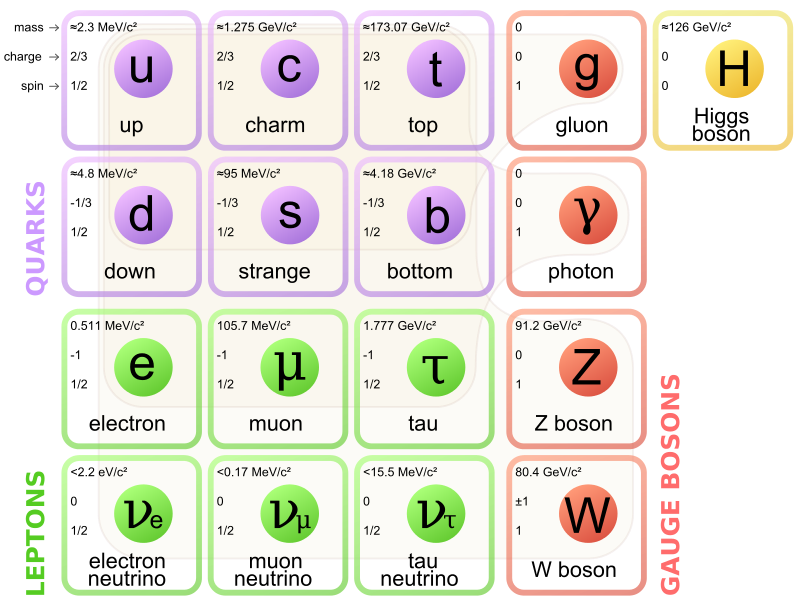
\includegraphics[width=0.7\textwidth]{figures/CLIC/StandardModel.png}
  \caption{The building blocks of matter according to the Standard
    Model~\cite{wikipediaParticles}.}
  \label{fig:standardmodel}
\end{figure}

Today, the Standard Model is the best theory describing the subatomic
world. However, it does not answer questions like the nature of dark
matter. This theory also predicts the existence of the Higgs boson
which gives the mass to all particles. It was experimentally observed
in 2012 by the ATLAS~\cite{Aad20121} and CMS~\cite{Chatrchyan201230}
experiments at CERN.

The weak and the electromagnetic forces are closely related to each
other and can be unified as the \textit{electroweak} interaction and
the equations describing the unification predict the force-carrying
particles (the photon, the W and Z bosons). All force-carrying
particles are described as being massless which is true for the
photon, but the W and Z bosons have a mass about 100 times larger than
that of the proton. To solve this problem, the Brout-Englert-Higgs
mechanism was introduced which suggests that the Higgs boson gives the
mass to the W and Z boson by interaction with a Higgs field.

The Higgs boson can be produced in a particle collider by collisions
between highly energetic particles. Heavy particles, like the Higgs
boson, are occasionally produced and detected by a particle
detector. The most important parameters of a particle collider are its
center-of-mass energy, determining the types of particles that can be
studied or discovered, and its instantaneous luminosity, determining
the event rates. For a given process, the cross section is a measure
of quantum mechanical probability for interaction and it depends on
the fundamental physics. Therefore, the observed number of events for
a given process depends on the integrated luminosity over the
operation time of the collider and the cross section of the
process. The Standard Model predicts different mechanisms to produce
the Higgs boson and the cross section is very small. For example, in
LHC only 1 Higgs boson is produced per 10 billion collisions.

An electron-positron collider allows to perform precision measurements
by colliding beams made of elementary particles. With elementary
particles, the center-of-mass energy and the polarisation of the
colliding particles can be selected precisely. Unlike proton-proton
collisions at the LHC experiments, there is no underlying event from
proton remnants. The complicated environment of a hadron machine makes
the measurements of the fundamental properties of the Higgs boson very
hard. The added value of an electron-positron collider would be to
measure in great details the Higgs mass and its total decay width, its
spin-parity quantum numbers, its couplings to fermions and gauge
bosons and also its self couplings that allows for the reconstruction
of the scalar potential that is responsible of electroweak symmetry
breaking~\cite{Linssen:1425915}.


CLIC is foreseen to be built and operated in three stages with
center-of-mass energies of $380\,\gev$, $1.5\,\tev$ and $3\,\tev$ as
shown in \cref{fig:CLICstaging}~\cite{Felzmann:2157041}. The site
studies have shown that CLIC could be placed near CERN
underground. For each stage, to increase the center-of-mass energy,
more accelerating modules will be needed, making the accelerator
longer. The site length for $3\,\tev$ will be 50~km.

\begin{figure}[htbp]
  \centering
  \includegraphics[width=0.7\textwidth]{figures/CLIC/staging.pdf}
  \caption{The three implementation stages of CLIC near CERN with
    center-of-mass energies of $380\,\gev$, $1.5\,\tev$ and
    $3\,\tev$~\cite{Felzmann:2157041}.}
  \label{fig:CLICstaging}
\end{figure}

The different energy stages at CLIC allow for maximising the
luminosity performance and physics potential for high precision
measurements of Standard Model physics (e.g. Higgs, top) as well as
new physics potentially discovered at the $13\,\tev$ LHC.

The first energy stage allows for studying the Standard Model Higgs
physics and top-quark physics with the possibility to perform a t\={t}
threshold scan. This stage gives the possibility to perform
model-independent cross-section
measurements~\cite{Abramowicz:2016zbo}. The second energy stage
provides direct sensitivity to many physics beyond the SM (BSM)
models. With larger Higgs statistics, rare processes such as t\={t}H
and double Higgs production can be measured. Finally, the third energy
stage provides the best sensitivity to new physics, the double-Higgs
production and allows for improving the measurements of the Higgs
self-coupling and HHWW quartic
coupling. \cref{fig:HiggsProductionMechanisms} shows different
mechanisms to produce the Higgs boson at CLIC.

\begin{figure}[htbp]
  \centering
  \begin{tikzpicture}
    % \node[anchor=south west,inner sep=0] (image) at
    % (0,0){\includegraphics[page=43, trim=30mm 235mm 25mm 30mm, clip,
    %   width=\textwidth]{figures/CLIC/clicCDR.pdf}};

    \node[anchor=south west,inner sep=0] (image) at
    (0,0){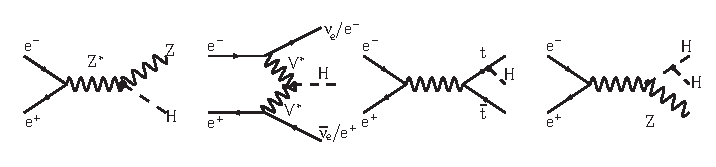
\includegraphics[width=\textwidth]{figures/CLIC/HiggsProductionMechanism.pdf}};
    
    \begin{scope}[x={(image.south east)},y={(image.north west)}]
      
      \node[below, color=black] at (0.14, 0.1)
      {e\textsuperscript{+}e\textsuperscript{-}$\rightarrow$ZH};

      \node[below, color=black] at (0.4, 0.1)
      {e\textsuperscript{+}e\textsuperscript{-}$\rightarrow$H$\nu_{e}\bar{\nu_{e}}$};

      \node[below, color=black] at (0.6, 0.1)
      {e\textsuperscript{+}e\textsuperscript{-}$\rightarrow$t\={t}H};

      \node[below, color=black] at (0.87, 0.1)
      {e\textsuperscript{+}e\textsuperscript{-}$\rightarrow$ZHH};
      
      % \draw[help lines,xstep=.1,ystep=.1] (0, 0) grid (1,1);
      % \foreach \x in {0,1,...,9} { \node [anchor=north] at (\x/10,0) {0.\x}; }
      % \foreach \y in {0,1,...,9} { \node [anchor=east] at (0,\y/10) {0.\y}; }
      
    \end{scope}
    
  \end{tikzpicture}
  \caption{Standard Model Higgs boson production mechanisms at
    CLIC~\cite{Linssen:1425915}.}
  \label{fig:HiggsProductionMechanisms}
\end{figure}

The cross sections to produce a Higgs with a mass of $M_H = 126\,\gev$
as a function of the center-of-mass energy $\sqrt{s}$ are given in
\cref{fig:corssSectionH125}. Below $\sqrt{s}$ of $\sim500\,\gev$, the
HZ mechanism is dominant. For higher energies, the
H$\nu_{e}\bar{\nu_{e}}$ mechanism dominates.

\begin{figure}[htbp]
  \centering
  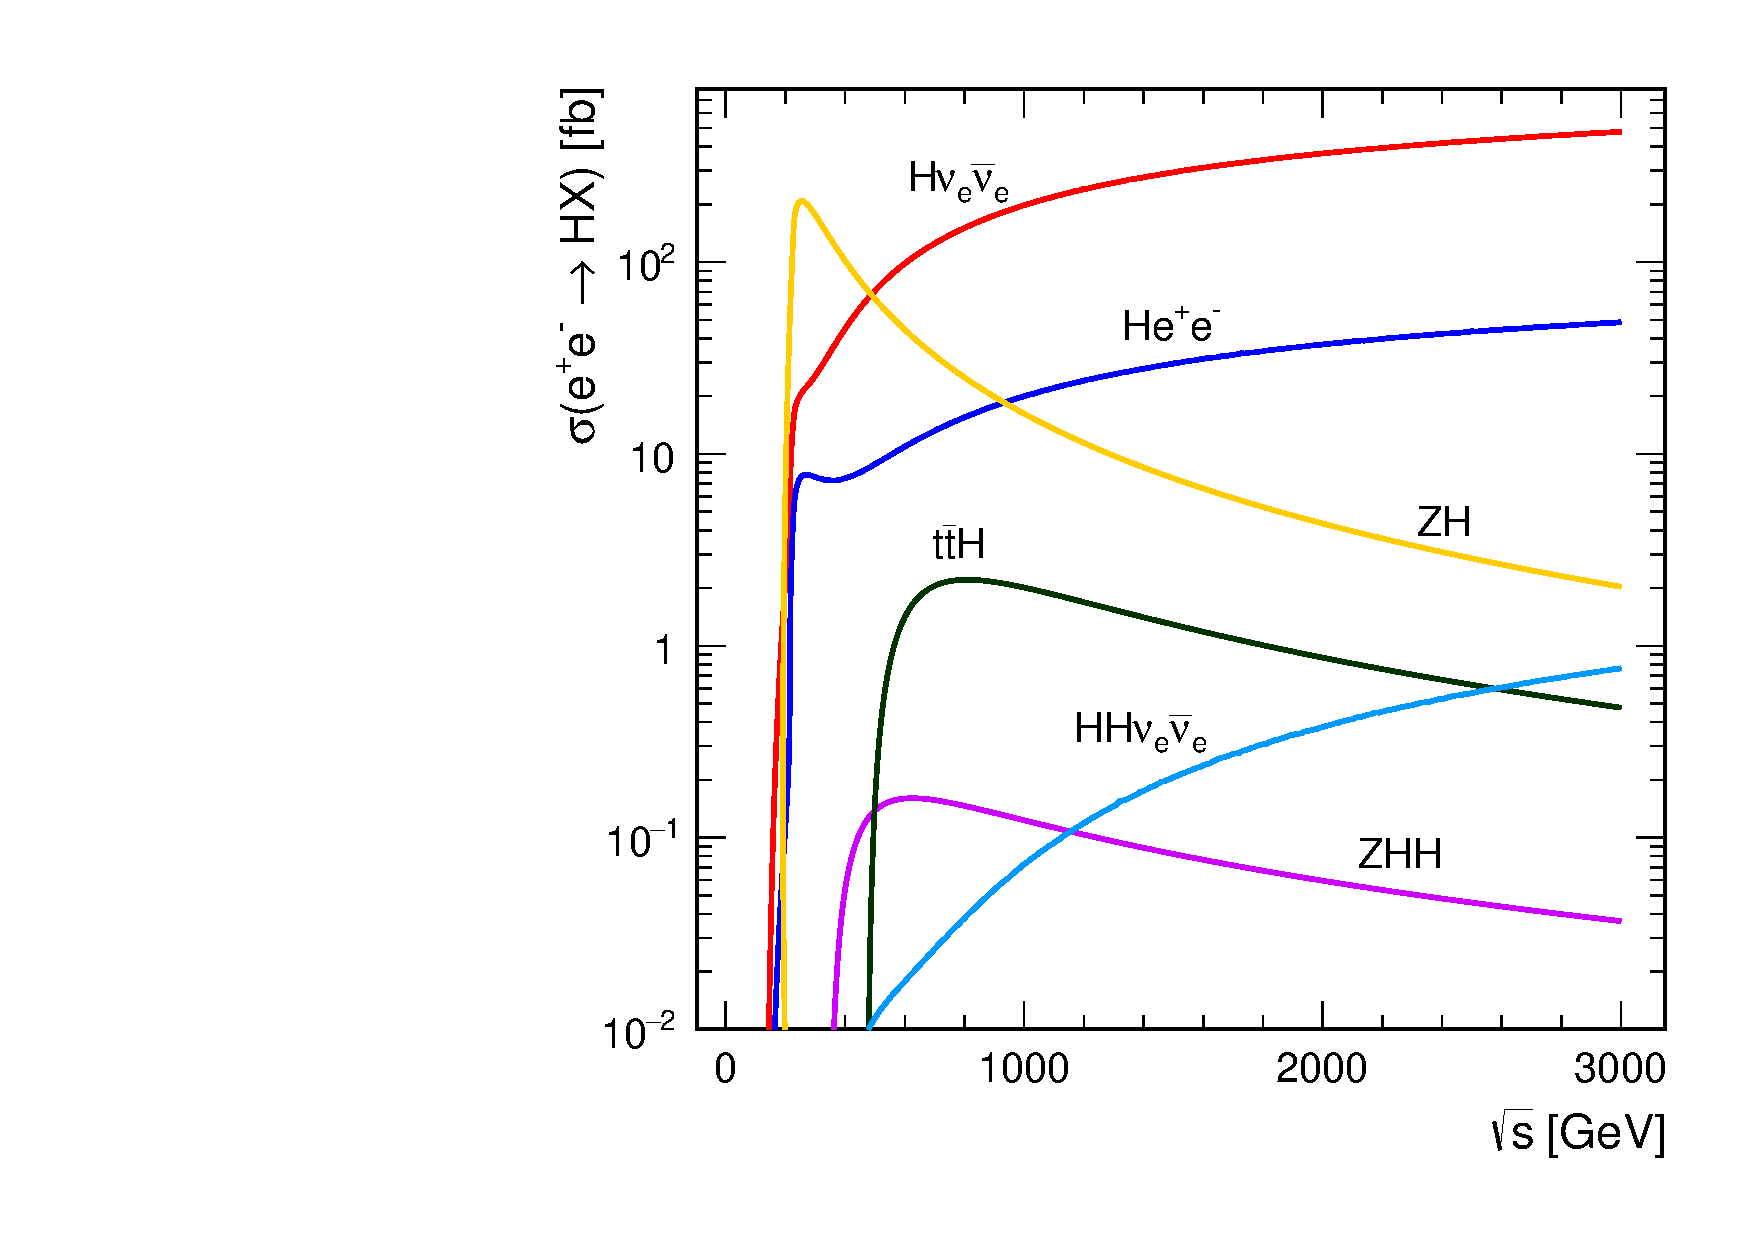
\includegraphics[width=0.5\textwidth]{figures/CLIC/xsec_vs_cme.pdf}
  \caption{Cross sections for the main Higgs production mechanisms for
    a $M_H~=~126\,\gev$ Higgs boson as a function of the e$^+$e$^-$
    center-of-mass energy in a lepton collider. These values
    correspond to unpolarised beams and the effect of beamstrahlung is
    not included~\cite{Felzmann:2157041}.}
  \label{fig:corssSectionH125}
\end{figure}

Final states with heavy quark flavours are important in many physics
channels, such as the Higgs and the top. The identification of the
heavy quarks is performed through the measurement of the displaced
vertices and the vertex detector has a crucial role in these
measurements as described in the following chapters.


\section{The CLIC accelerator}

The schematic layout of the CLIC accelerator complex at
$\sqrt{s}=3\,\tev$ is shown in \cref{fig:CLIC_accelerator}. The
electron and positron beams are accelerated on a linear trajectory and
collide in the central region (at the interaction point), where the
CLIC detector is placed. Each linac is fed by a drive-beam generation
complex.

\begin{figure}[htbp]
  \centering
  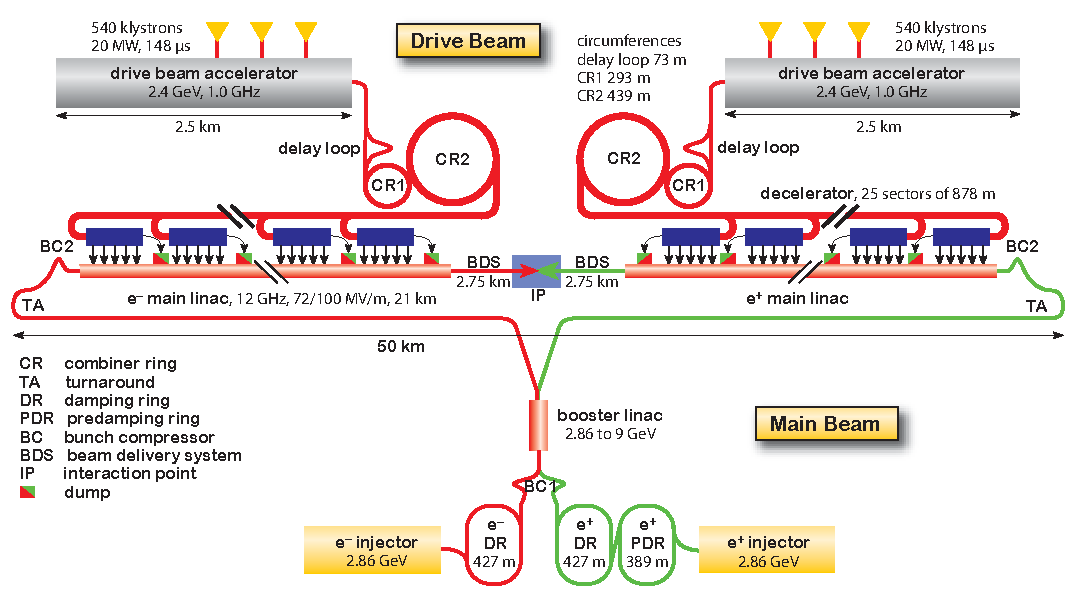
\includegraphics[width=\textwidth]{figures/CLIC/CLIC-layout2015pub.pdf}
  \caption{Schematic layout of the CLIC accelerator complex at
    $\sqrt{s}=3\,\tev$. Each linac is fed by a drive-beam generation
    complex~\cite{Felzmann:2157041}.}
  \label{fig:CLIC_accelerator}
\end{figure}

To limit the length of the accelerator, the accelerating field has to
be as high as possible. The accelerating gradient is chosen to be
100~MV/m. This leads to the use of copper cavities at room temperature
instead of superconducting cavities since the latter have an
intrinsically limited maximum field. The copper cavities are fed with
radio frequency (RF) power at a very high frequency of
$12\,\gigahertz$ to generate the high accelerating field. This leads
to a total RF peak power of 9.2~TW for both linacs. Since maintaining
such high power levels is not possible for very long, the duration of
the bunch train is limited to 156~ns with a repetition frequency of
50~Hz.


Traditionally, klystrons are used in accelerators to provide the RF
power to the main beam. However, for CLIC, klystrons are not directly
used to accelerate the main beam since a large number of them would be
needed and their efficiency would be too low at $12\,\gigahertz$. A
two-beam acceleration scheme is used to reach the nominal collision
energy. A drive beam is running in parallel to the main beam. The
drive beam has a low energy of $2.4\,\gev$ and a high current of
100~A. It is used to transfer the energy of the klystrons to the main
beam which has a lower current and higher energy. Power Extraction and
Transfer Structures (PETS) are special RF devices which extract the
power of the drive beam by decelerating the beam. The extracted energy
is then provided to the main beam. CLIC is divided into sectors with
an average length of 878~m and each section accelerates the main beam
by $\approx62\,\gev$.


\cref{tab:NominalMachineParams} summarises the nominal beam parameters
for the $3\,\tev$ CLIC and $13\,\tev$ LHC. An instantaneous luminosity
$\mathcal{L}$ of a few $10^{34}$~\inversecmsquaredsec insures a
sufficient amount of data collected in a reasonable amount of
time. The beam sizes at the interaction point of CLIC have to be
extremely small in order to achieve the desired luminosity. The RF
pulse duration limits the number of bunches and the bunch-crossing
separation. CLIC and LHC have similar luminosity despite the
differences in beam parameters.

\begin{table}[htbp]
  \centering
  \caption{Nominal beam parameters for CLIC at $\sqrt{s}=3\,\tev$ and
    LHC at $\sqrt{s}=13\,\tev$.}
  \label{tab:NominalMachineParams}
  \begin{tabular}{l c c}
    \toprule
    & CLIC at $\sqrt{s}=3\,\tev$ & LHC at $\sqrt{s}=13\,\tev$\\
    \midrule
    Colliding particles & electron-positron & proton-proton \\
    Instantaneous luminosity $\mathcal{L}$ & $6\times10^{34}$ \inversecmsquaredsec & $1\times10^{34}$ \inversecmsquaredsec \\
    Bunch-crossing separation & 0.5~ns & 25~ns \\
    Bunches per train & 312 & Not applicable \\
    Train duration & 156~ns & Not applicable \\
    Train repetition & 50~Hz & Not applicable \\
    IP size in x / y / z directions & 45~nm / 1~nm / $44\,\micron$ & $15\,\micron$ / $15\,\micron$ / 50~cm \\
    \bottomrule
  \end{tabular}
\end{table}

\subsection{Beam-induced backgrounds}
\label{sec:beamInducedBackgrounds}

The small beam sizes at CLIC cause strong electromagnetic radiation
(Beamstrahlung) from the electron and positron bunches in the field of
the opposite beam. The generation of Beamstrahlung photons leads to a
reduction of the available centre-of-mass energy $\sqrt{s}$ of the
e\textsuperscript{+}e\textsuperscript{-} collisions. The interactions
of Beamstrahlung photons produce lepton pairs and hadrons at low polar
angles which are mostly contained in the
beam-pipe~\cite{Dannheim:1443516}. In the inner detector layers,
incoherently produced electron-positron pairs ($\sim60$ particles per
bunch crossing) and $\gamma\gamma\rightarrow$hadrons events ($\sim54$
particles per bunch crossing) are the dominant backgrounds.

The electron-positron pairs produced at low polar angles have very
small transverse momentum. The occupancies in the innermost layers of
the detector can be reduced to an acceptable level by optimising the
inner and forward detector regions. The beam-pipe walls have to be
placed outside of the high-rate region. The inner detectors have to be
shielded from the backscattered particles which originate from the
forward region.

The $\gamma\gamma\rightarrow$hadrons interactions produce particles
with a higher transverse momentum spectrum and a more central
polar-angle distribution. This results in large rates of background
particles reaching the outer detector layers. In each train, at most
one interesting physics event is expected along with $\sim1000$
hadronic background events.

Hit time stamping on the level of 1 to 10~ns in all sub-detectors is
needed in order to separate the physics from the background events.

The exposure to radiation of the main detector elements is expected to
be small compared to high-energy hadron-colliders.

\section{The CLIC detector}
\label{sec:CLICdetector}

To cover the CLIC physics potential, a detector concept is under
development. The physics goals set challenging requirements on the
design of the detector. Simulation tools are crucial for the design,
development as well as the optimisation of the detector model.

The experimental conditions due to the beam-induced background (see
\cref{sec:beamInducedBackgrounds}), set the most demanding
requirements at the highest collision energy. Therefore, the detector
model is mainly optimised for the $3\,\tev$ CLIC.

\cref{fig:CLIC_detector_concept} shows the CLIC detector model as
implemented in simulations. The overall length and height of the
detector are 11.4~m and 12.9~m respectively. It is composed of several
sub detectors. The vertex detector is the closest to the IP and
consists of pixelated silicon detectors. It is followed by the main
tracker which is also a silicon-based detector. After the tracking
systems, fine grained calorimeters are used: the silicon-tungsten
electromagnetic calorimeter (ECAL) and the steel hadronic calorimeter
(HCAL). The superconducting coil surrounds the calorimeters to provide
a magnetic field of 4~T to deflect the trajectory of charged
particles. The tracking detectors use the radius of curvature to
measure the momentum of charged particles. In the very forward region,
the luminosity calorimeter (LumiCal) is used to reconstruct precisely
the energy and angle of electrons and positrons obtained from Bhabha
events and employed for the luminosity
measurements~\cite{Abramowicz:2010bg}. The beam calorimeter (BeamCal)
is used for electron tagging by the identification of high energy
electrons~\cite{Abramowicz:2004me}. Finally the iron yoke surrounds
the whole detector and is instrumented for the identification of
muons.


\begin{figure}[htbp]
  \centering
  \begin{tikzpicture}
    \node[anchor=south west,inner sep=0] (image) at
    (0,0){\includegraphics[width=0.62\textwidth]{figures/CLIC/CLICdp_Top_view_HD_temp.pdf}};
    \begin{scope}[x={(image.south east)},y={(image.north west)}]
      %% \draw[help lines,xstep=.1,ystep=.1] (0, 0) grid (1,1);
      %% \foreach \x in {0,1,...,9} { \node [anchor=north] at (\x/10,0) {0.\x}; }
      %% \foreach \y in {0,1,...,9} { \node [anchor=east] at (0,\y/10)
      %% {0.\y}; }
      \node[draw, text width=2cm] at (-0.2, 0.9) {Ultra low-mass vertex detector};
      \draw[->,line width=1pt, color=black](-0.02, 0.9) -- (0.5, 0.5);

      \node[draw, text width=2cm] at (-0.2, 0.7) {Main tracker, silicon based};
      \draw[->,line width=1pt, color=black](-0.02, 0.7) -- (0.35, 0.55);

      \node[draw, text width=2cm] at (-0.2, 0.5) {Forward region with LumiCal \& BeamCal};
      \draw[->,line width=1pt, color=black](-0.02, 0.45) -- (0.25, 0.49);

      \node[draw, text width=2cm] at (-0.2, 0.2) {Fine grained
        calorimetry optimised for Particle Flow Analysis (PFA)};
      \draw[->,line width=1pt, color=black](-0.02, 0.2) -- (0.3, 0.3);

      \node[draw, text width=2cm] at (1.15, 0.15) {Return yoke (Fe) with detectors for muon ID};
      \draw[->,line width=1pt, color=black](1, 0.1) -- (0.8, 0.1);

      \node[draw, text width=2cm] at (1.15, 0.79) {Solenoid magnet: B=4~T};
      \draw[->,line width=1pt, color=black](1, 0.79) -- (0.8, 0.79);
      

      \node[color=black] at (0.5, 0.05) {11.4~m};
      \draw[<->,line width=1pt, color=black](0.03, 0.02) -- (0.97,
      0.02);

      \node[color=black] at (1.1, 0.5) {12.9~m};
      \draw[<->,line width=1pt, color=black](0.99, 0.01) -- (0.99, 0.99);
      
      % \draw[help lines,xstep=.1,ystep=.1] (0, 0) grid (1,1);
      % \foreach \x in {0,1,...,9} { \node [anchor=north] at (\x/10,0) {0.\x}; }
      % \foreach \y in {0,1,...,9} { \node [anchor=east] at (0,\y/10) {0.\y}; }
      
    \end{scope}
  \end{tikzpicture} 
  \caption{Schematic layout of the CLIC detector
    concept~\cite{CLICdetUnpublishedNote}.}
  \label{fig:CLIC_detector_concept}
\end{figure}

\subsection{Requirements for the vertex-detector}
\label{sec:VXD_requirements}

The main goal of the CLIC vertex detector is the efficient tagging of
heavy quarks through the precise measurement of the displaced
vertices. To achieve this goal, Monte Carlo
simulations~\cite{Linssen:1425915} have shown that a high-momentum
term in the transverse impact-parameter resolution of
$a\approx5\,\micron$ and a multiple-scattering term of
$b\approx15\,\micron$ are needed using the canonical parametrisation:

\begin{equation}
 \sigma(d_0)=\sqrt{a^2+b^2 \cdot\gev^2/(p^2 \text{sin}^3\theta)} \; ,
  \label{eq:canonicalParam}
\end{equation}

where $p$ is the momentum of the particle and $\theta$ is the polar
angle with respect to the beam axis.

To meet these requirements, a multi-layer barrel and endcap pixel
detector with an inner radius of $\approx$30~mm with a geometrical
coverage extending down to low polar angles
($\theta_{min}\approx8^{\circ}$) is needed. For the beam-pipe and for
each of the detection layers a material budget of $\approx0.2\%$ of a
radiation length (X\textsubscript{0}) is considered. Sensors with a
single-point resolution of $\approx3\,\micron$ operating in a magnetic
field of 4~T are required.

In the innermost layers, an occupancy of $\approx3\%$ due to the
beam-induced backgrounds is expected~\cite{Dannheim:1443516}. To
separate these backgrounds from physics events, a time slicing of the
hits with an accuracy of $\approx10$~ns is required. To achieve this
precise time stamping, hybrid detectors (where sensors and electronics
are separately manufactured and later combined) are preferred since
they provide more advanced timing measurement technologies.

In comparison to the current pixel detectors in the LHC experiments,
the expected radiation level in the region of the CLIC vertex detector
is moderate. For the inner-detector layers a total $1\,\mev$
neutron-equivalent fluence of less than
$10^{11}$~neq/cm\textsuperscript{2}/year and a total ionising dose of
less than 1~kGy are expected~\cite{Dannheim:1443516}.

The aim of the vertex detector R\&D is to achieve the required
single-point resolution with pixels of size
$\approx25\,\micron\times25\,\micron$ with $50\,\micron$ thick sensors
coupled to $50\,\micron$ thick readout ASICs with pulse-height
measurement capability. The constraint on the material budget implies
no active cooling elements can be placed inside the vertex
detector. To limit the maximum power dissipation of the readout
electronics to $\approx50~\text{mW/cm}^2$, forced air-flow cooling and
power pulsing (i.e. turning off most components on the readout chips
during the 20~ms gaps between bunch trains) are foreseen.

\section{Flavour-tagging performance at CLIC}
\label{sec:flavourTagging}

The precision physics measurements require excellent flavour-tagging
performance of the CLIC vertex detector. Different vertex detector
geometries have been studied for
CLIC~\cite{AlipourTehrani:1742993,Tehrani:2015tla}. This section
presents the impact of the geometry on the flavour-tagging performance
in simulations.

A first geometry designed for the CLIC vertex detector is shown in
\cref{fig:disksGeom}. It contains 5 layers in the barrel and 4 disks
in the endcap region. Since forced airflow cooling is foreseen for
CLIC as illustrated in Figure~\cref{fig:cooling}, a spiral arrangement
for the modules in the endcap regions has been implemented instead of
disks, allowing the air to flow through the vertex detector.

\begin{figure}[htbp]
  \centering
  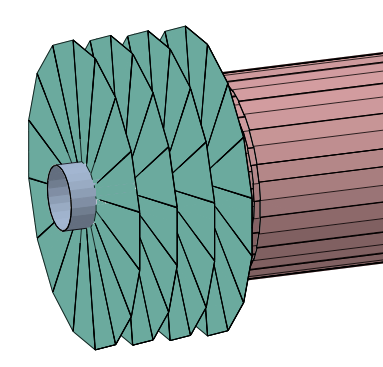
\includegraphics[width=0.4\textwidth]{figures/CLIC/cdr.png}
  \caption{The schematic view of the disks geometry with 5
    single-sided layers in the barrel region and 4 single-sided disks
    in the endcap region.}
  \label{fig:disksGeom}
\end{figure}

The physics performance of the geometries described in
Table~\ref{tab:geometries} and illustrated in
Figure~\ref{fig:geometries} have been studied in simulations.


The multi-variate LCFIPlus flavour-tagging
package~\cite{website:LCFIPlus} is used to assign each jet category
with a beauty (b) and charm (c) probability. The fake rates of
separating the charm and beauty jets from each other and from light
flavour (LF) jets are being investigated.

The detector models in simulation consider the single-point resolution
of the sensors ($\sim3\,\micron$) and include layer thicknesses based
on constraints from an engineering model of the mechanical support and
the air cooling system~\cite{AlipourTehrani:1742993}.


\begin{table}[htbp]
  \caption{Vertex detector geometries implemented in simulations.}
  \begin{center}
    \begin{tabular}{ l c c c }
      \hline
      Geometry & Barrel layers & Endcap layers & Material budget \\ \hline \hline
      \emph{spirals} (Figure~\ref{fig:SpiralsGeometry}) & 5 single-sided & 4 single-sided & $0.1\%X_{0}$ per single-sided layer  \\ %\hline 
      \emph{double\_spirals} (Figure~\ref{fig:doubleLayer}) & 3 double-sided & 3 double-sided & $0.2\%X_{0}$ per double-sided layer  \\ %\hline
      \emph{double\_spirals\_v2} & 3 double-sided & 3 double-sided & $0.4\%X_{0}$ per double-sided layer  \\ \hline  
    \end{tabular}
  \end{center}
  \label{tab:geometries}
\end{table}


\begin{figure}[htbp]
  \begin{subfigure}[b]{0.33\textwidth}
    \centering
    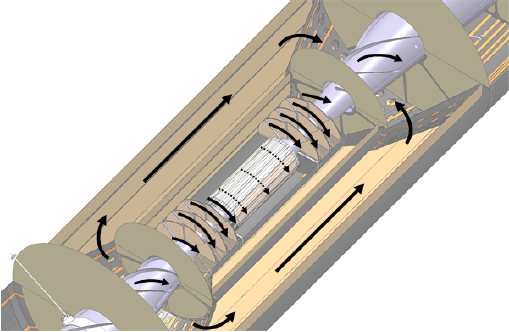
\includegraphics[width=\textwidth]{figures/CLIC/Cooling.png}  
    \caption{}
    \label{fig:cooling}
  \end{subfigure}~
  \begin{subfigure}[b]{0.33\textwidth}
    \centering
    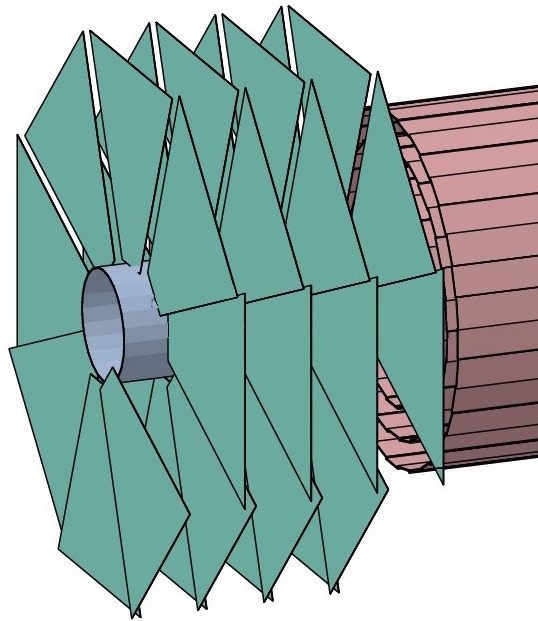
\includegraphics[width=0.65\textwidth]{figures/CLIC/single_spiral.jpg}
    \caption{}
    \label{fig:SpiralsGeometry}
  \end{subfigure}~
  \begin{subfigure}[b]{0.25\textwidth}
    \centering
    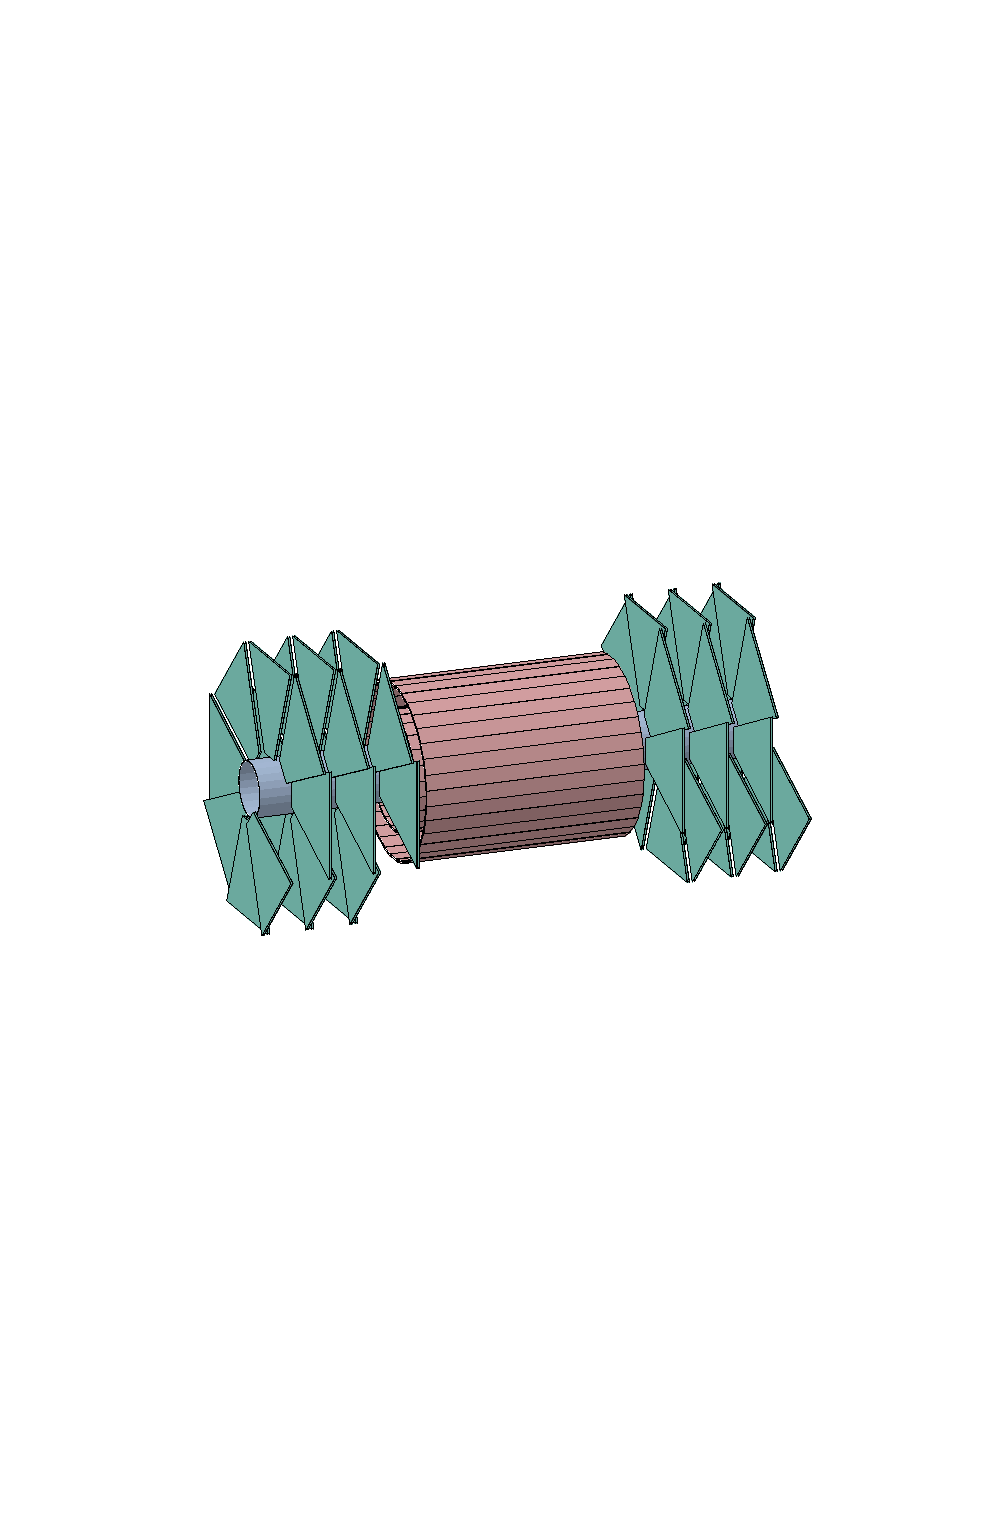
\includegraphics[trim = 32mm 98mm 85mm 106mm, clip, width=0.65\textwidth]{figures/CLIC/double_spiral.pdf} \\
    
\includegraphics[width=1.5\textwidth]{figures/CLIC/double_layer_module.png} 
    \caption{}
    \label{fig:doubleLayer}
  \end{subfigure}
  \caption{(a)~Sketch showing the airflow cooling strategy within the
    vertex detector~\cite{DuarteRamos:1572989}. (b)~Schematic view of
    the vertex detector for the \emph{spirals} geometry. (c)~Schematic
    view of the vertex detector for the
    \emph{double\_spirals(\_v2)}. In the \textsc{GEANT4}
    simulations~\cite{Agostinelli:2002hh}, a double-sided layer is
    implemented as two silicon sensors on top of each other with an
    overall thickness of
    \SI{2}{\milli\meter}. From~\cite{Tehrani:2015tla}.}
  \label{fig:geometries}
\end{figure}

The performance of the flavour tagging depends on the jet energy and
polar angle: dijet events with different center-of-mass energies,
$\sqrt{s}$, having polar angles of
$10^{\circ} \leq \theta \leq 90^{\circ}$ with a uniform distribution
in azimuthal $\phi$ angles are considered. Initial state radiation
(ISR) and beamstrahlung (BS) were switched off during the event
generation and hence the final-state quarks are in a back-to-back
configuration. For each jet flavour, energy and angle, 80000 events
are used for the following processes: e$^+$e$^-$ $\rightarrow$ b\={b},
c\={c}, u\={u}, d\={d}, s\={s}. The boosted decision tree (BDT)
classifiers are trained using 50\% of the generated events and the
other 50\% are used for testing the performance of the flavour
tagging.

\cref{fig:DisksPerformance} shows the dependence of the
flavour-tagging performance on the jet polar angle in the
\textit{disks} geometry for jets in dijet events at
$\sqrt{s}=200\,\gev$. \cref {fig:DisksPerformance_btag} shows the fake
rate of recognising beauty jets as charm jets versus the
beauty-tagging efficiency. For dijet events at $\theta=40^{\circ}$,
for a b-tagging efficiency of $80\%$, the probability to misidentify
charm quarks as beauty quarks is
$\sim5\%$. \cref{fig:DisksPerformance_ctag} shows the fake rate of
recognising charm jets as beauty jets versus the charm-tagging
efficiency. As expected, the b-tagging performance is better than the
c-tagging performance. However, CLIC allows for a higher charm tagging
performance compared to the LHC experiments.

\begin{figure}
  \begin{subfigure}[b]{0.49\textwidth}
    \centering
    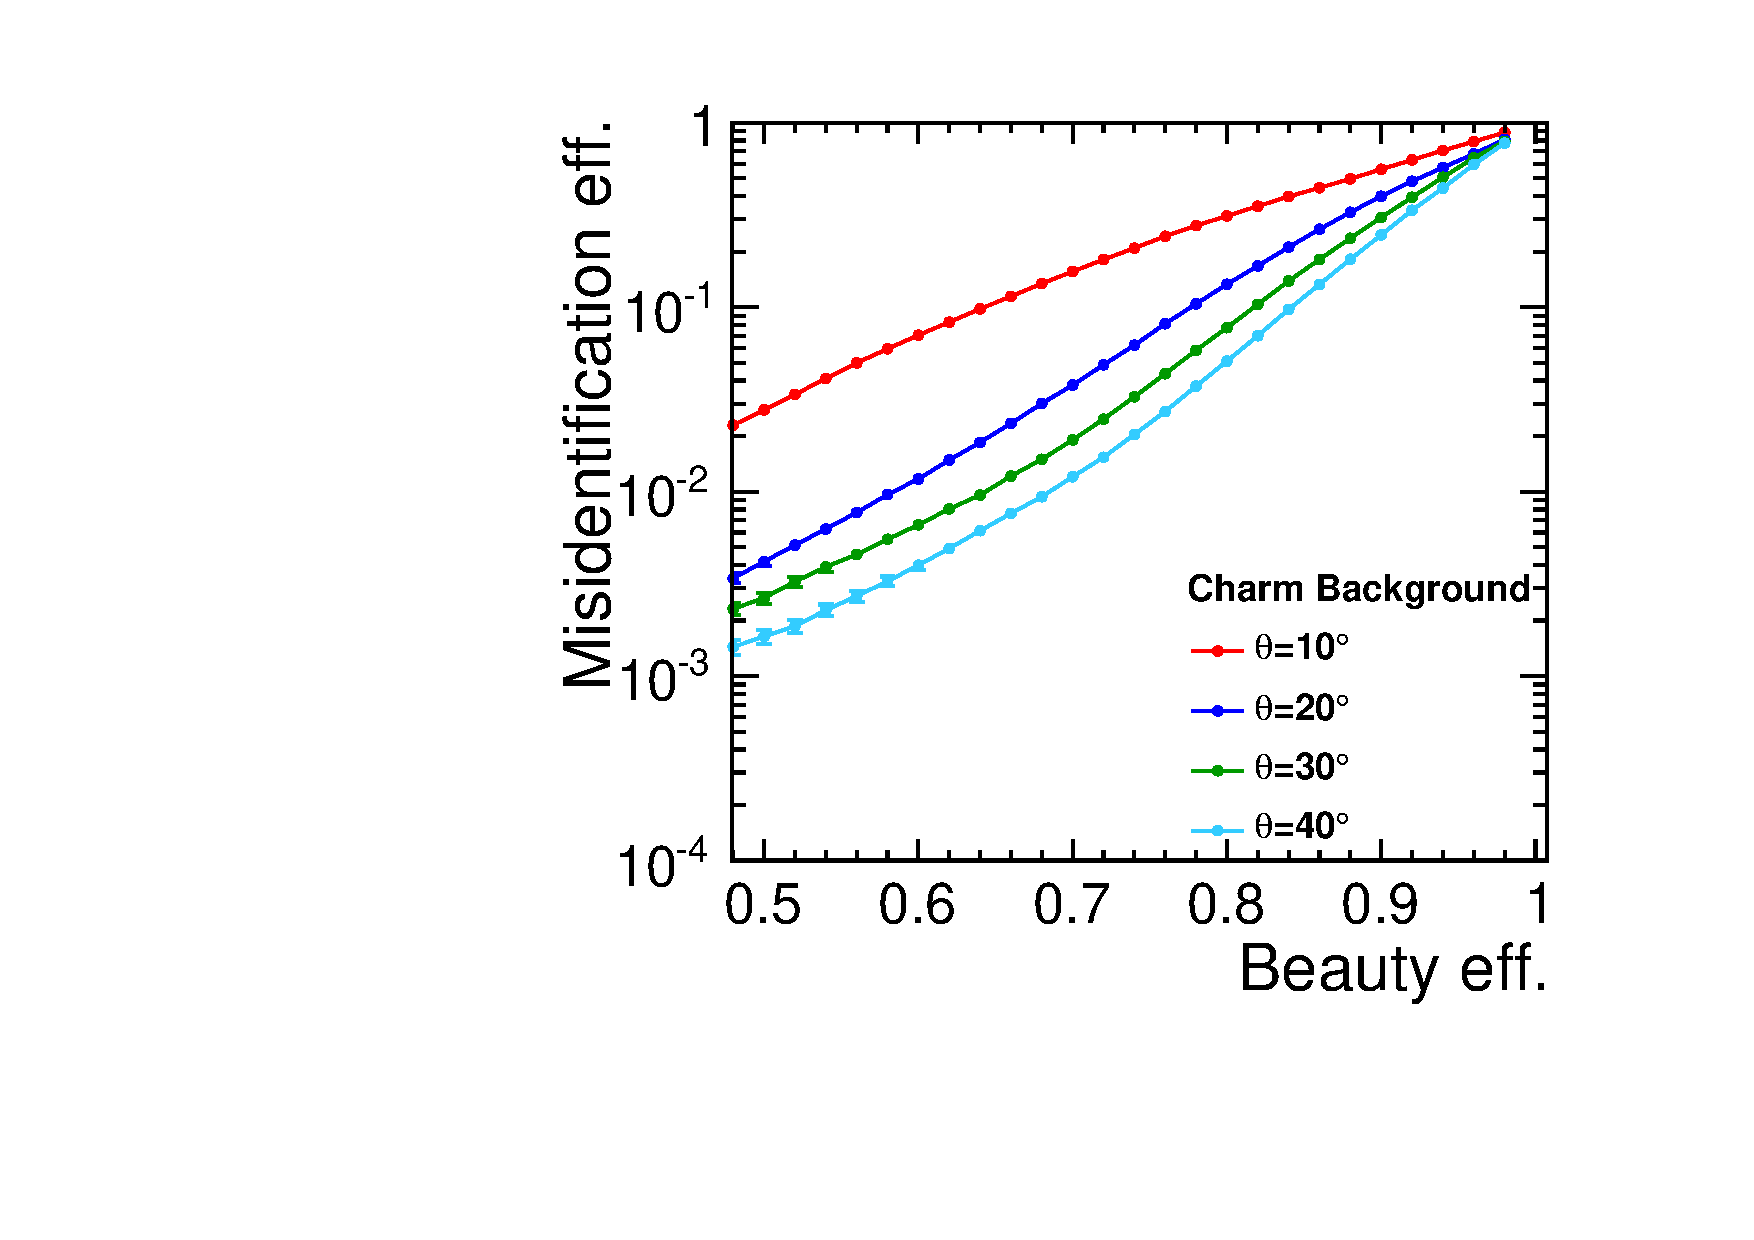
\includegraphics[width=\textwidth]{figures/CLIC/allAngles_CLIC_SiD_CDR_Beauty_Charm_200.pdf}
    \caption{}\label{fig:DisksPerformance_btag}
  \end{subfigure}\hfill
  \begin{subfigure}[b]{0.49\textwidth}
    \centering
    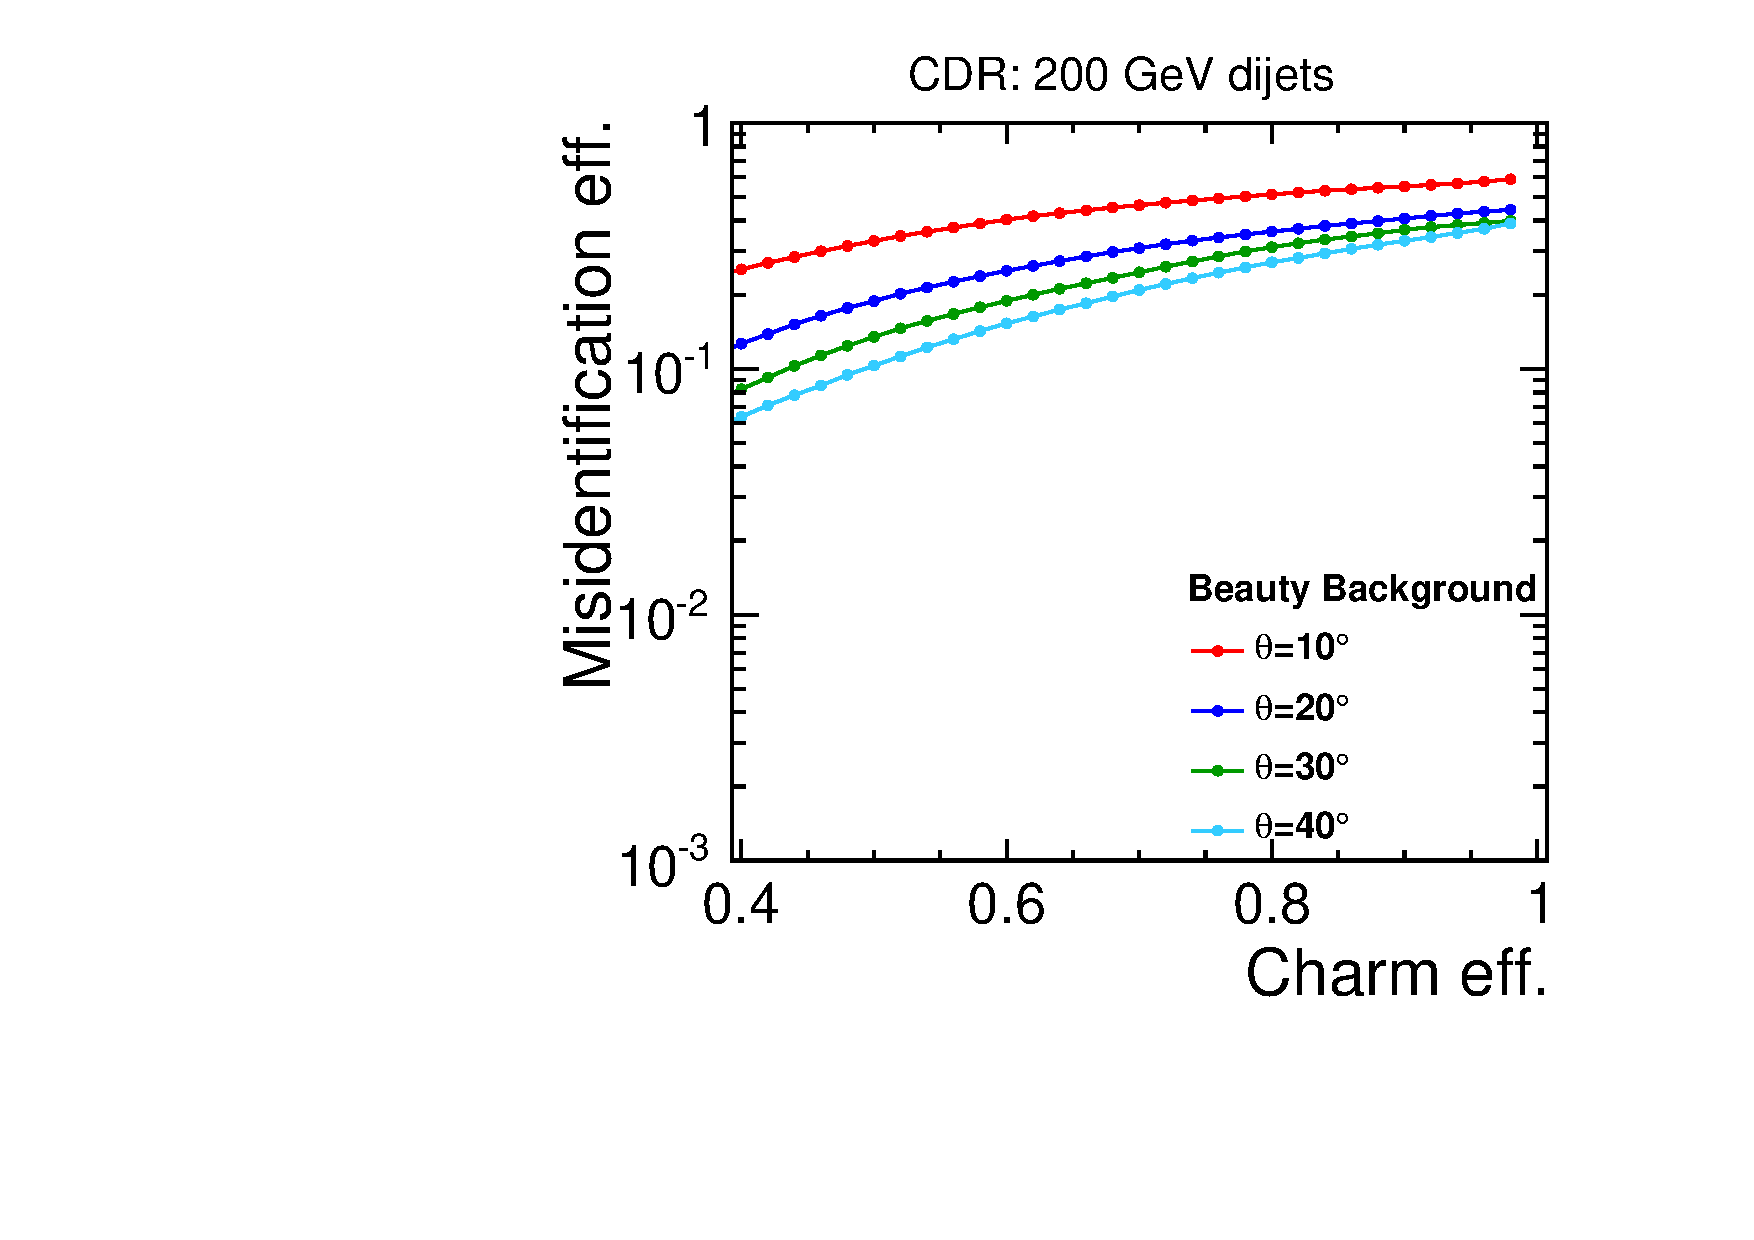
\includegraphics[width=\textwidth]{figures/CLIC/allAngles_CLIC_SiD_CDR_Charm_Beauty_200.pdf}
    \caption{}\label{fig:DisksPerformance_ctag}
  \end{subfigure} 
  \caption{(a) b-tag and (b) c-tag efficiency for jets in dijet events
    at $\sqrt{s}=200\,\gev$ with different polar angles for the
    \textit{disks} geometry~\cite{AlipourTehrani:1742993}.}
  \label{fig:DisksPerformance}
\end{figure}

The flavour-tagging performance for the different vertex detector
geometries as shown in \cref{fig:geometries} is summarised in
\cref{fig:performance} where the fake rate of recognising charm and
light flavour jets as beauty jets is plotted versus the b-tag
efficiency.

The \emph{spirals} and \emph{disks} have a similar flavour-tagging
performance except for jets at $\theta=40^{\circ}$ (see
Figure~\ref{fig:spiral_disks}), which corresponds to the transition
between the vertex endcaps and the barrel region, where the
beauty-tagging performance is up to $20\%$ worse using the
\emph{spirals} geometry (compared to disks). With the spiral
configuration, the number of sensitive layers becomes dependent on the
azimuthal angle $\phi$ and fewer layers can be hit in certain ranges
of $\phi$. The performance degradation caused by this $\phi$
dependence can be mitigated by increased $\phi$ overlap in future
geometry implementations.

The performance of the \emph{spirals} and the \emph{double\_spirals}
is very similar as shown in Figure~\ref{fig:spiral_doubleSpirals}.
The \emph{double\_spirals\_v2} geometry is a more realistic version of
the \emph{double\_spirals} geometry, taking into account the material
used for the mechanical support of the sensors and also for the
cables. As shown in Figure~\ref{fig:doubleSpirals_doubleSpirals}, the
misidentification probability increases by $\sim$35\% due to the
increased material.


\begin{figure}[htbp]
  \begin{subfigure}[b]{0.33\textwidth}
    \centering
    \begin{tikzpicture}
      \node[anchor=south west, inner sep=0] (image) at (0,0){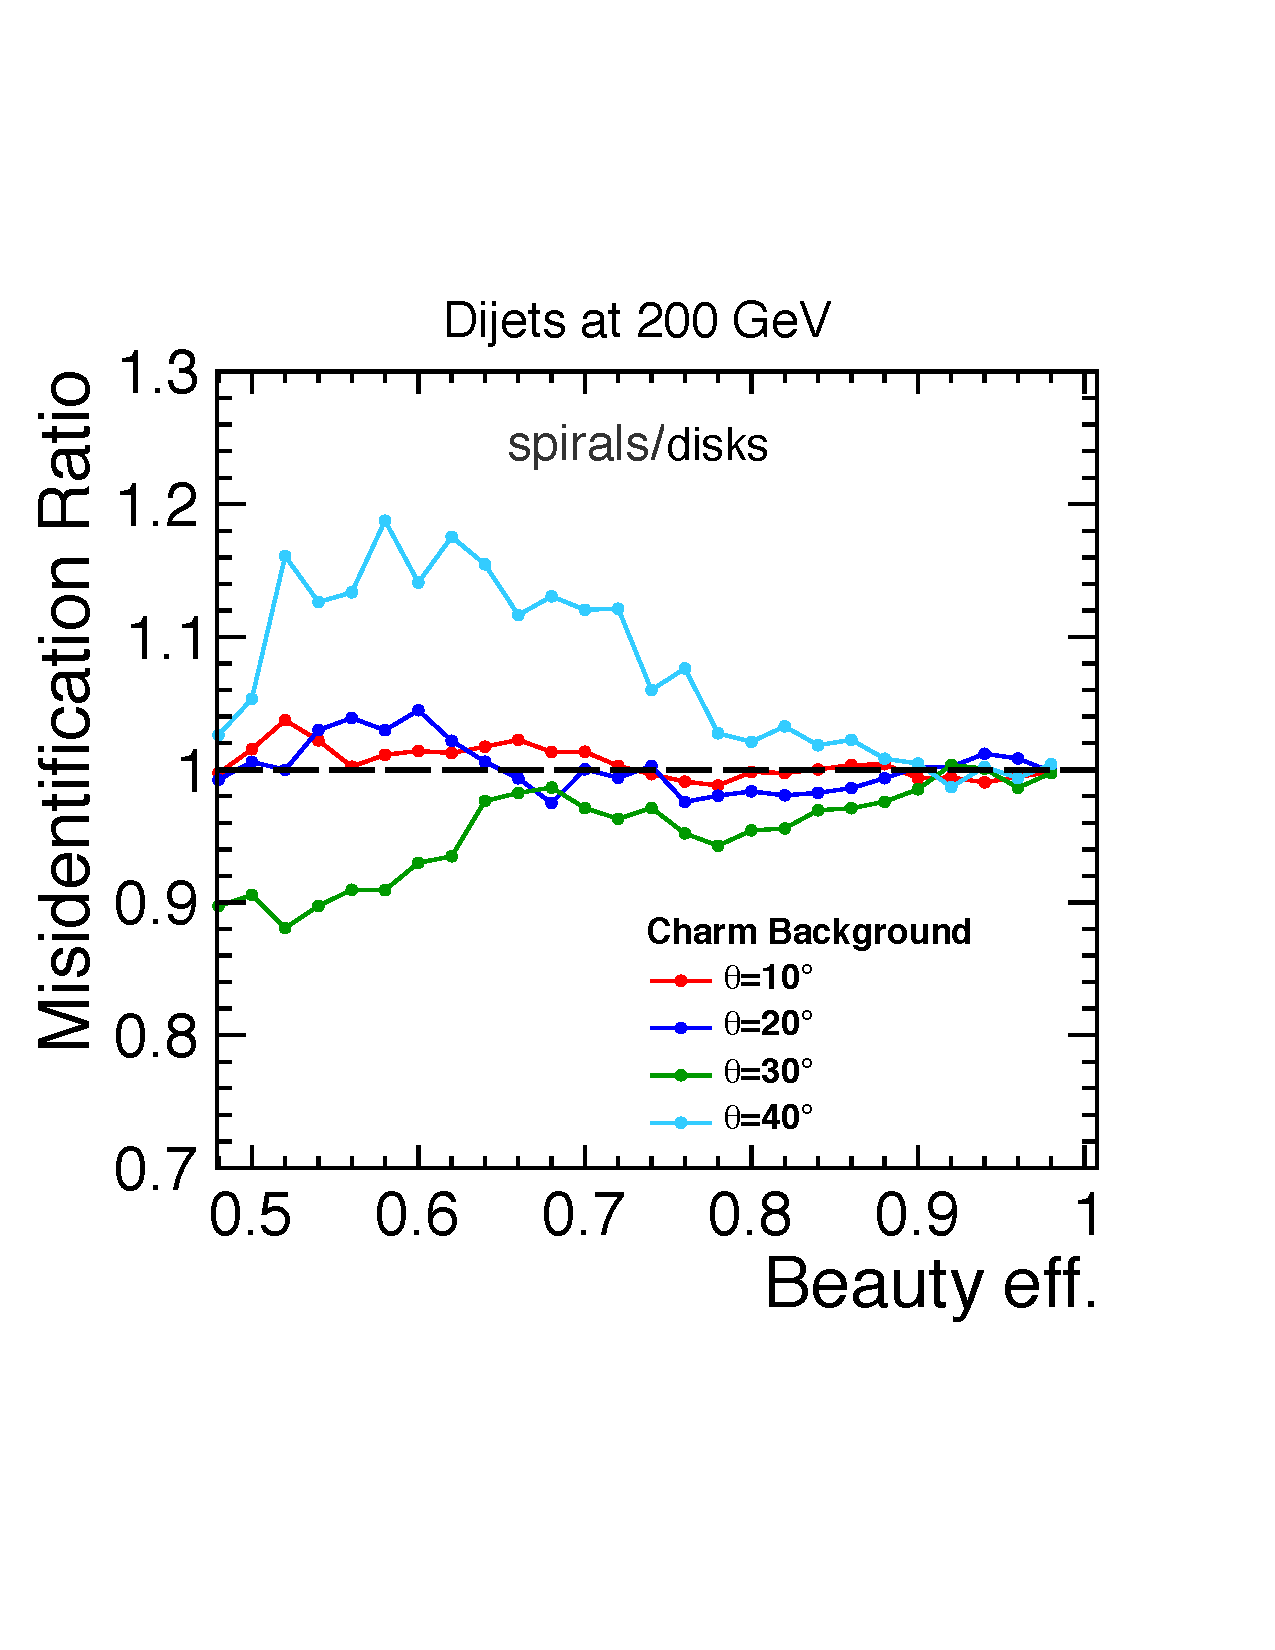
\includegraphics[trim = 5mm 50mm 20mm 20mm, clip, width=\textwidth]{figures/CLIC/200GeV_Ratio_allAngles_spirals_CDR_B_C.pdf}};
      \draw  (1.8, 1.5) node {\textbf{CLICdp}};
    \end{tikzpicture}
    \caption{}
    \label{fig:spiral_disks}
  \end{subfigure}~
  \begin{subfigure}[b]{0.33\textwidth}
    \centering
    \begin{tikzpicture}
      \node[anchor=south west, inner sep=0] (image) at (0,0){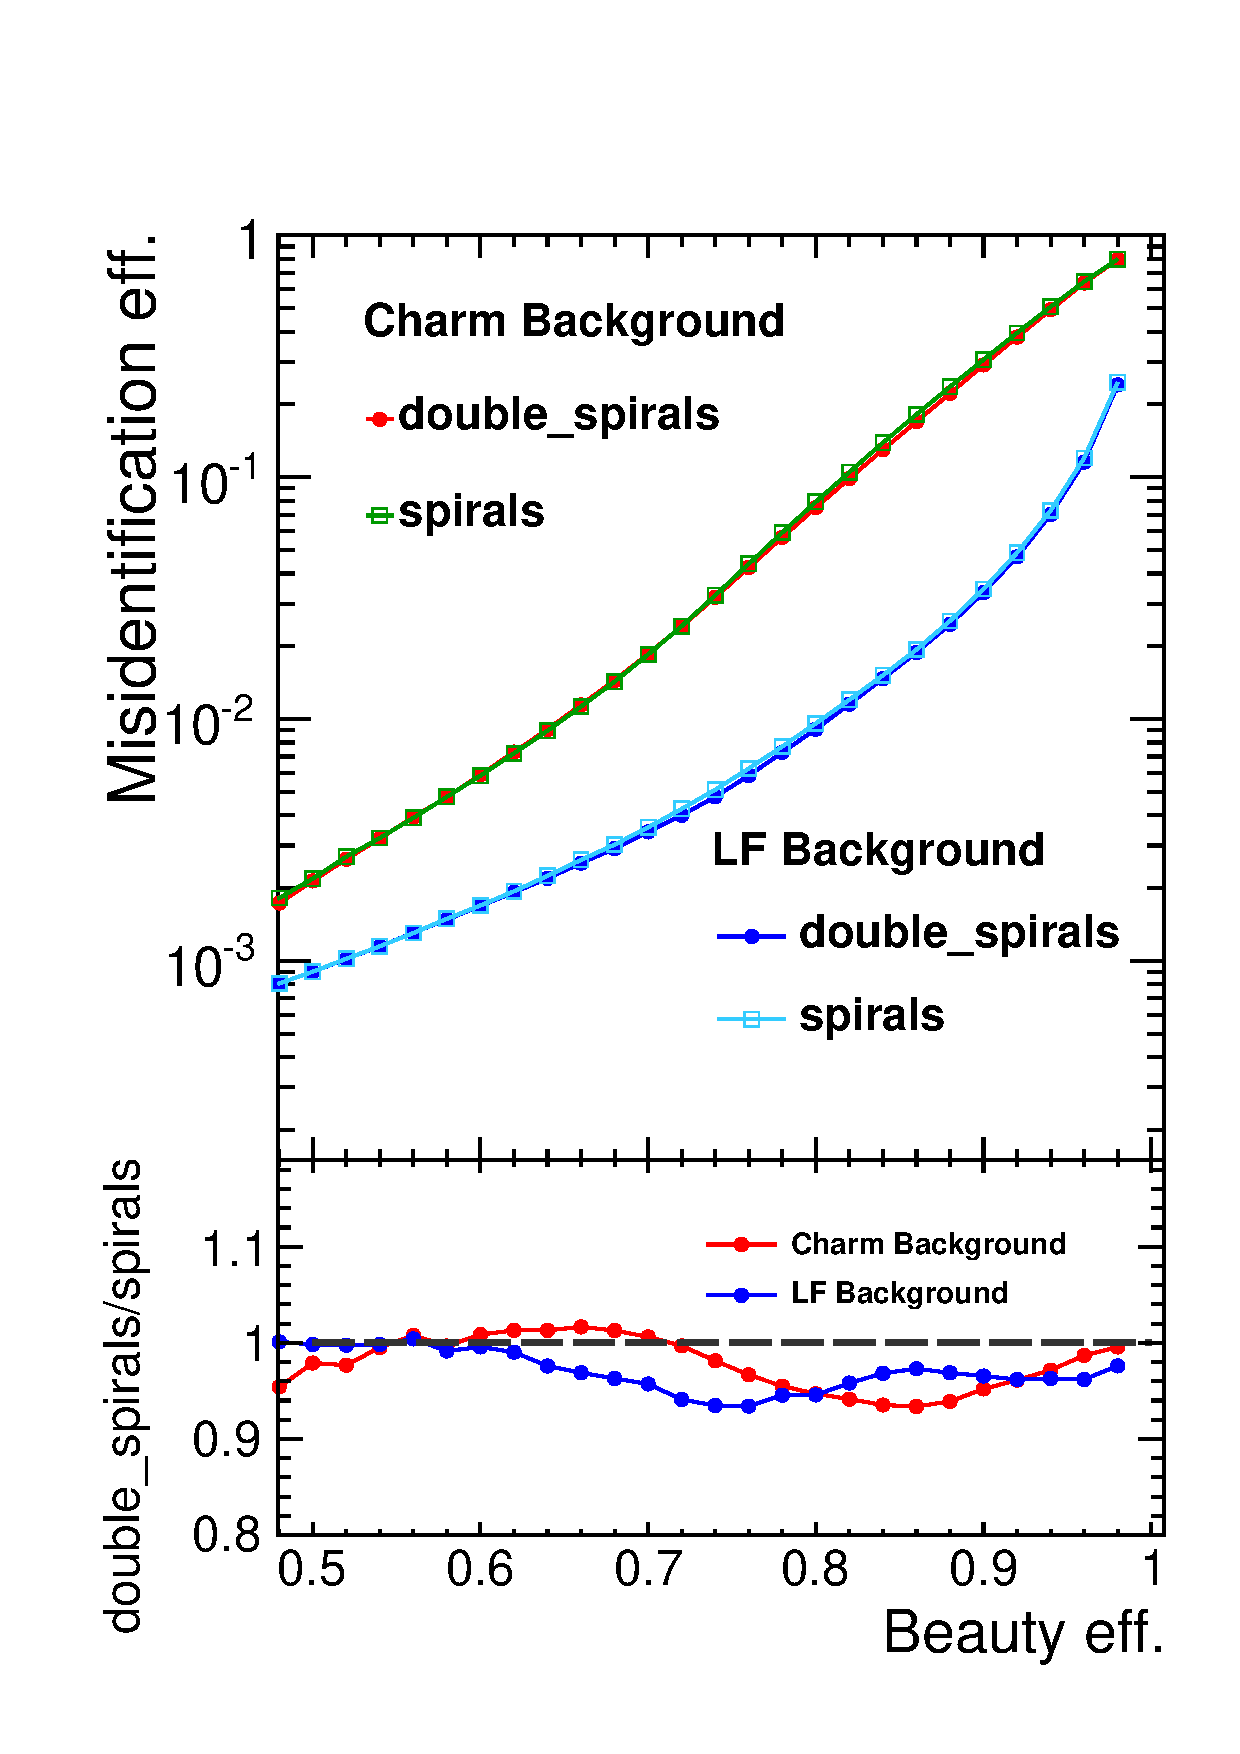
\includegraphics[width=\textwidth]{figures/CLIC/general_200_Beauty.pdf}};
      \draw (1.8, 2.8) node {\textbf{CLICdp}};
    \end{tikzpicture}
    \caption{}
    \label{fig:spiral_doubleSpirals}
  \end{subfigure}~
  \begin{subfigure}[b]{0.33\textwidth}
    \centering
    \begin{tikzpicture}
      \node[anchor=south west, inner sep=0] (image) at (0,0){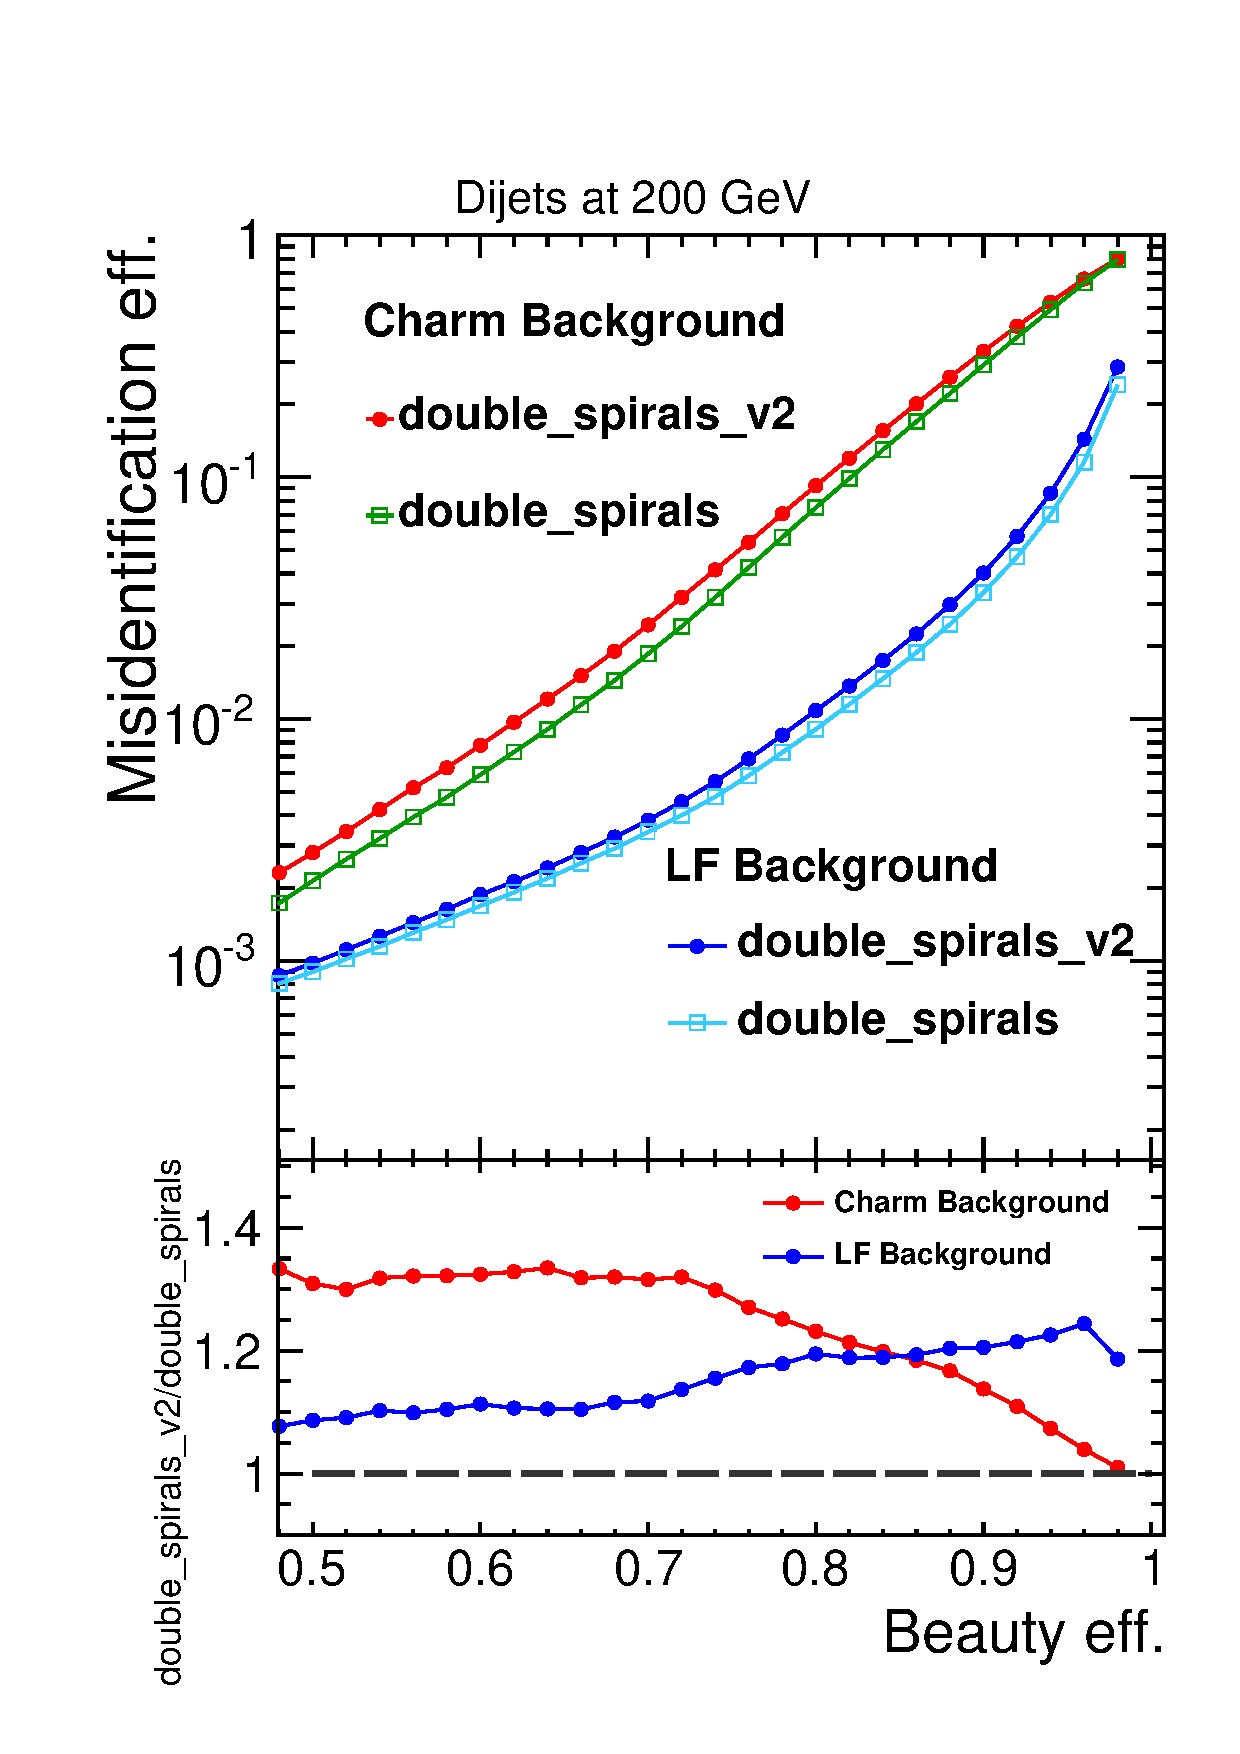
\includegraphics[width=\textwidth]{figures/CLIC/heavy_general_200_Beauty.pdf}};
      \draw (1.8, 2.8) node {\textbf{CLICdp}};
    \end{tikzpicture}
    \caption{}
    \label{fig:doubleSpirals_doubleSpirals}
  \end{subfigure}
  \caption{Beauty-tagging performance for dijet events at
    \SI{200}{\giga\electronvolt}. (a)~Comparison between \emph{disks}
    and \emph{spirals} in terms of the ratio of the misidentification
    probabilities for charm background. (b)~Comparison of the
    beauty-tagging performance between the \emph{spirals} and
    \emph{double\_spirals} geometries. (c)~Comparison of the
    beauty-tagging performance between the \emph{double\_spirals} and
    \emph{double\_spirals\_v2} geometries. For (a) the
    misidentification ratio for each polar angle is shown
    separately. For (b) and (c), dijet events with a mixture of polar
    angles between \SI{10}{\degree} and \SI{90}{\degree} are
    considered. From~\cite{Tehrani:2015tla}.}
  \label{fig:performance}
\end{figure}

A detector model for CLIC is under development which takes into
account the progressing engineering studies. The spiral arrangement of
the modules in the vertex endcaps allows to use airflow cooling which
has the potential to reduce the material budget
significantly. Double-sided modules provide more sensitive layers with
the same amount of support material as single-sided modules. The
overall results show that the implemented geometries are similar in
terms of the flavour-tagging performance for simulated dijet
events. The impact of a spiral arrangement of the modules in the
endcap region remains similar to the disks. The amount of material, on
the other hand, was found to have a large impact on the performance.

The following chapters focus on the R\&D of the pixel detectors in the
vertex detector with high-resolution and very low material budget in
order to achieve high flavour-tagging performance as required by the
precision physics to be measured at CLIC.



% \section{Summary}
% \label{sec:summary_CLIC}

% The CLIC detector model for simulations is under development with the
% requirements set by the precision physics to be measured. With these
% requirements, it allows for identification of beauty and charm quarks
% and this is possible with a vertex detector with a high spatial
% resolution and very low material budget to limit the multiple
% scatterings. This thesis focuses on the R\&D of the pixel detectors in
% the vertex detector with high-resolution and very low material budget.

% ============================================================================== 
% planning for the chapter
% ============================================================================== 
% Accelerator (two-beam acceleration), CLIC detector concept, picture of
% the full detector (3 pages)

% \section{Requirements for the CLIC vertex detector}
% motivation for pixel detectors in high-energy physics (flavour-tagging
% plots), requirements, design, technical challenges
% (cooling/mechanics), Beam induced backgrounds, Radiation damage in the
% vertex detector (3 pages).


% \section{Flavour tagging at CLIC}
% say motivation of this thesis $\Rightarrow$ provide input for the
% digitiser (1 page) and the detector simulation software.
